%************************************************
\chapter{\emph{an example}}
\label{chapter:an_example}
%************************************************

\begin{figure}[bth]
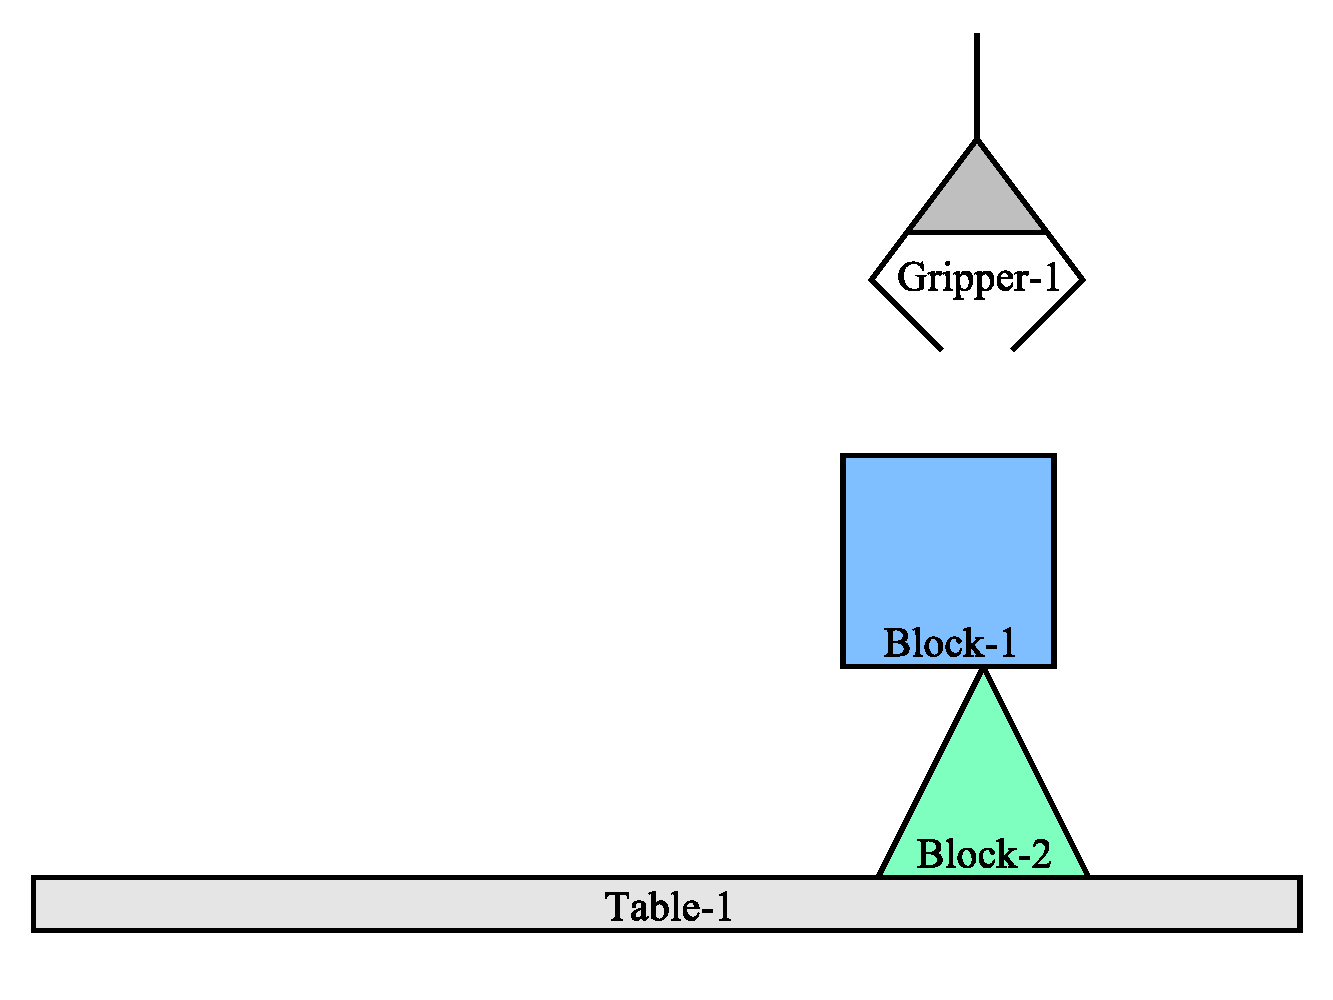
\includegraphics[width=10cm]{gfx/blocks_world_example_failure} \\ \medskip
\caption{A failure to stack two blocks.}
\label{figure:example_of_failure}
\end{figure}

I begin my explanation of my thesis by describing the example
situation pictured in \autoref{figure:example_of_failure}:
\begin{quote}
There is a table.  Some blocks are on the table.  The blocks are of
different shapes and colors.  One of the blocks is a green triangle.
Another block is a blue square.  A hand can move around, picking up
and putting down blocks.  Plans can be made for the hand to arrange
the blocks into different configurations.  Plans can be followed that
can result in failures.  For example, putting the square on top of the
triangle might fail to stack the two blocks because the square might
fall off of the triangle.  These failures can be thought of as
learning opportunities.  Through failures, better models of the
physical world can be learned.  Also through failures, better models
of planning can be learned.  Learning different planning strategies
for different physical situations is a reflective form of learning.
My thesis is to describe SALS, the implementation of a model of
layered reflective learning.
\end{quote}
I begin with a non-technical description of the model in plain
English.  Next, I transition to thinking of the model as a simulation.
I use mathematical set notation to describe the model as a simulation.
Finally, I describe how this mathematical simulation is automated on a
concurrent computer, SALS, the substrate for accountable layered
systems.

At the end of \autoref{part:the_model}, I explain the modelling
assumptions that I make in transitioning to the mathematical notation
of \autoref{part:simulating_the_model}.  Using this notation, I
explain how this model can be used to reduce the complexity of search
algorithms.  In \autoref{part:the_implementation}, I give an
explanation of how this simulation in implemented in SALS.  Finally,
in conclusion, I discuss promising directions for future research in
not only AI but also the other cognitive sciences, giving a plan for
how I see this model being extended to exhibit arbitrary
self-reflective strata.

